\documentclass[../dissertation.tex]{subfiles}

\begin{document}

\chapter{Critical Evaluation}

\label{chap:evaluation}

Here, a range of techniques are used to evaluate the newly proposed Neural-Q path tracer against the Expected Sarsa path tracer presented in Chapter \ref{chap:td_deep_sampling} on its ability to reduce noise in rendered images produced by Monte Carlo path tracing. The introduction of deep reinforcement learning for importance sampling light transport paths in Monte Carlo path tracing comes with a variety of benefits which are tested and discussed in detail. However, the methods viability in industry is currently found to be limited due to the time taken to evaluate a forward pass through an ANN.

\section{Experimental Setup}

A path tracing renderer was built from scratch which supported Algorithms \ref{alg:forward_path_tracing}, \ref{alg:expected_sarsa_pathtracer}, \ref{alg:neural_q_pathtracer} and was used to produce all rendered results seen in this thesis. The rendering engine used only OpenGL Mathematics library \cite{glm} for various operations that are common in the rendering pipeline, SDL2 \cite{sdl2} for displaying rendered images, and the Dynet neural network library \cite{dynet} for the Neural-Q path tracer implementation. Algorithms \ref{alg:forward_path_tracing}, \ref{alg:expected_sarsa_pathtracer}, \ref{alg:neural_q_pathtracer} were all accelerated on an Nvidia GPU by using the CUDA Toolkit \cite{cuda} to receive experimental results in an acceptable time. The reasoning for choosing Dynet over more commonly used neural networks libraries such as Tensorflow \cite{tensorflow2015-whitepaper}, was due to its ability to be easily compiled with the CUDA \verb|nvcc| compiler and it had a well documented C++ API. This was a requirement for the Neural-Q path tracer as tracing light paths, ANN inference, and ANN training are all performed on a Nvidia GPU via C++ API calls. All results were produced using a machine with an Intel i5-8600K CPU, Nvidia 1070Ti GPU and 16GB of RAM installed.\\

I developed four different scenes using Maya \cite{maya} and created a custom object importer to import the scenes into my path tracer renderer. A reference image of all four scenes is given in Figure \ref{fig:reference_scenes}, which have been rendered with 4096 sampled light rays per pixel using the default forward path tracing Algorithm \ref{alg:forward_path_tracing}. They are known as reference images as they have minimal visible noise, meaning the Monte Carlo approximations for each pixel's colour value has approximately converged. Due to path tracing accurately modelling physical light transport (see section \ref{sec:mc_pathtracing}), these images are the ideal case for which all other path tracing algorithms should aim to produce as closely as possible with as few samples as possible. 

% Insert reference images of four test scenes

\section{Assessing the reduction in image Noise for Monte Carlo Path Tracing}

\subsection{Quantifying the Reduction in Image Noise}

To quantify the amount noise within images rendered by a default forward path tracer, the Expected Sarsa path tracer, and the Neural-Q path tracer, I will use the Mean Absolute Percentage Error (MAPE) given in Equation \ref{eq:mape} \cite{muller2018neural}.

\begin{equation}
\label{eq:mape}
M = \frac{1}{N} \sum_{i=0}^{N-1} \left| \frac{A_i - F_i}{A_i} \right|
\end{equation}

\noindent
Where:
\begin{conditions}
N & The total number of pixels in the image\\
A_i & The $i$th pixel value in the reference image\\
F_i & The $i$th pixel value in the image whose noise is being quantified\\
\end{conditions}

The MAPE value can therefore be used to quantify the average difference between pixel values from an image rendered by each rendering technique with the same number of sampled light rays per pixel and the reference image. Therefore, a lower MAPE score is desirable for a rendered image as it means the image has a lower amount of noise.\\

%TODO Table presenting memory usage between two techniques for each scene & batch size needs to be mentioned somewhere

\begin{figure}[hbtp]
\begin{center}
\includegraphics[width=0.9\textwidth]{images/noise_reduction.png}    
\end{center}
\caption{A comparison of the default forward path tracer, Expected Sarsa path tracer, and the Neural-Q path tracer of their image noise for four different rendered scenes. All scenes were rendered with 128 samples per pixel. The score under each column in an image row corresponds to the MAPE score for each  path tracing algorithm for the particular scene.The Neural-Q and Expected Sarsa algorithms both used $144$ equally spaced directions to estimate the radiance distribution on a given point. The Neural-Q path tracer used the network described in \ref{sec:ann_architecture} for all fours scenes with a decaying $\epsilon$-\textit{greedy} policy start at $\epsilon =1$ with a decay of $\delta = 0.05$ applied after every pixel in the image has had a light path sampled through it once. The Expected Sarsa path tracer used just enough Irradiance Volumes (which varied depending on the scene) to facilitate a significant reduction in image noise in all four renders.}
\label{fig:mape_results_grid}
\end{figure}

\subsection{A Closer Inspection of Pixel Error Values}

By visual observation of the rendered images \ref{fig:mape_results_grid}, the type of noise present in the Expected Sarsa and Neural-Q path tracer's renders is quite different. In particular, the noise resulting from the Expected Sarsa path tracer are pixels with very high RGB values compared to that of their neighbours, which are commonly referred to as 'fireflies'  \cite{christensen2016path}. Whereas the noise present in the Neural-Q renders is more subtle, however its general presence can be clearly seen when comparing these renders to that of the reference image. In order to investigate this further I have provided histograms in Figure \ref{fig:histogram_errors} for the frequency of average RGB pixel error values of the rendered image compared to the reference image. Essentially, the greater the average RGB error for a particular pixel, the higher the amount of noise present in the pixel value estimate.

\begin{figure}[h]
\begin{center}
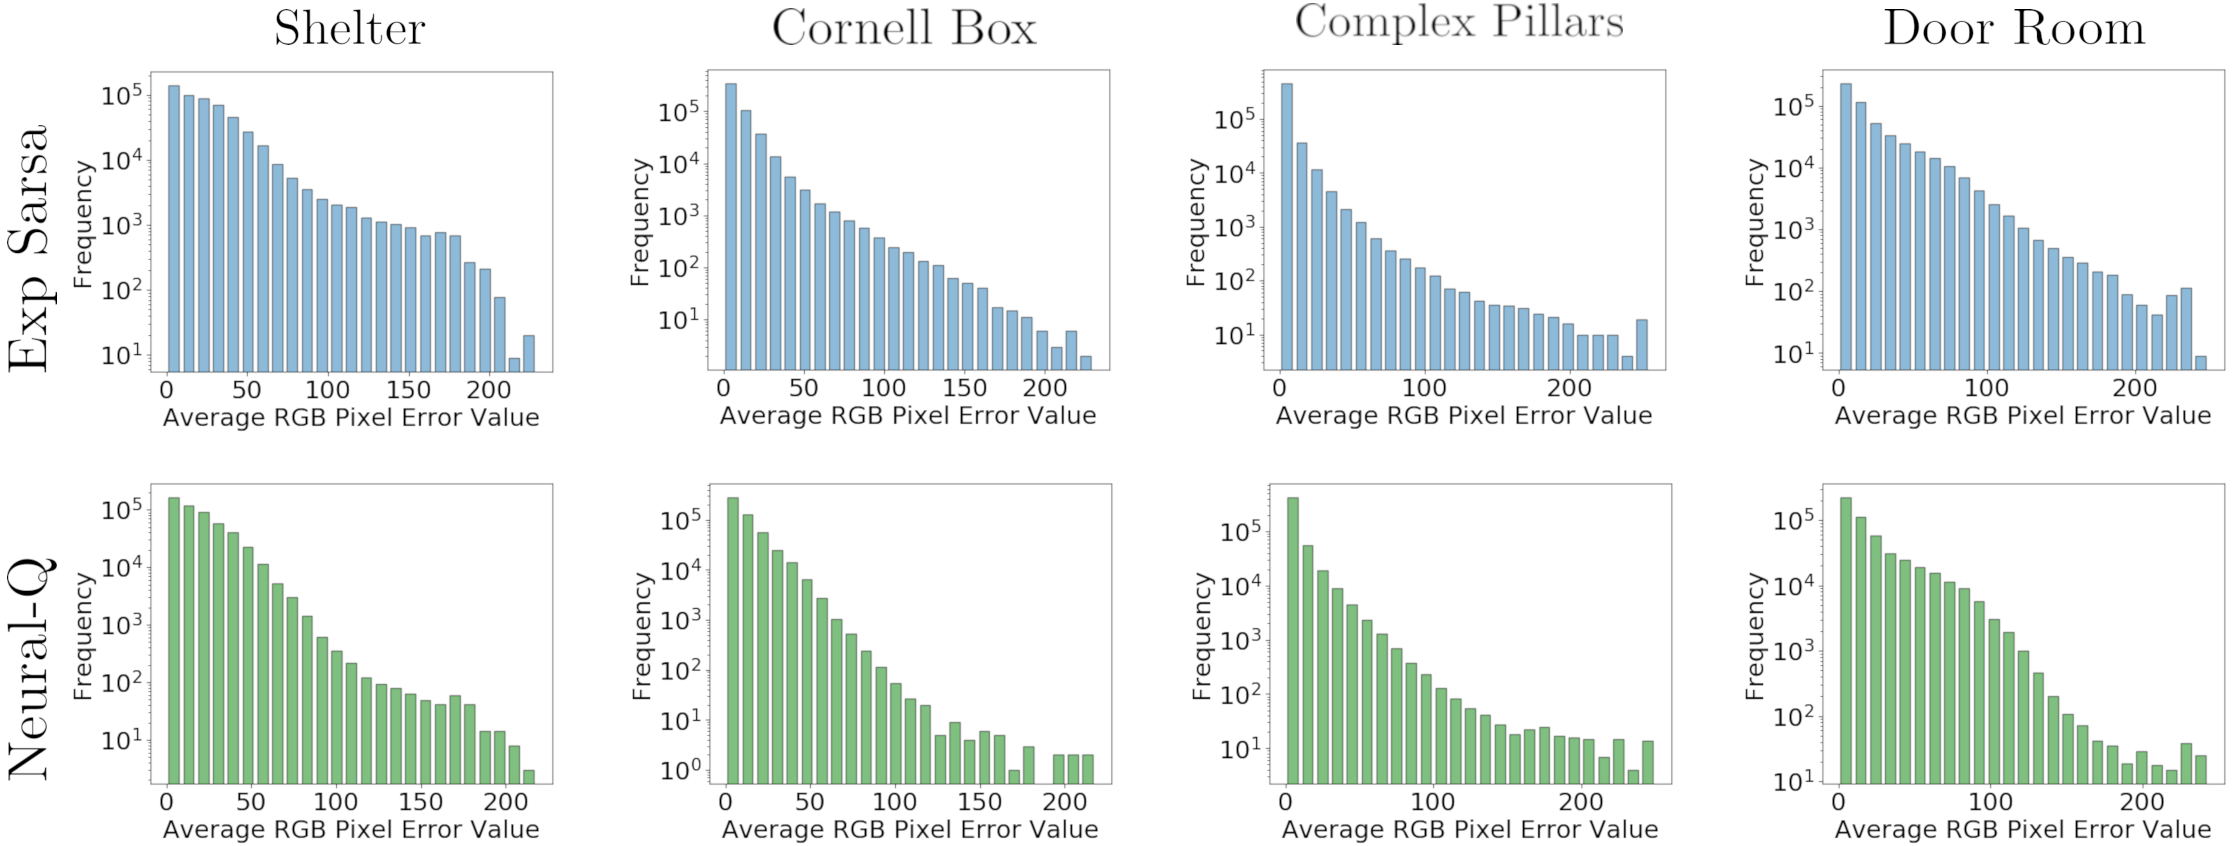
\includegraphics[width=0.99\textwidth]{images/noise_diff.png}    
\end{center}
\caption{Histograms for the average RGB pixel error values for all four rendered scenes using both the Expected Sarsa path tracer and the Neural-Q path tracer. Where the average RGB pixel error value is the average difference in all RGB colour channels between a pixel in the reference image, and the corresponding pixel in the image rendered by either the Expected Sarsa or Neural-Q path tracers. The histograms are based on the rendered images presented in Figure \ref{fig:mape_results_grid}.}
\label{fig:histogram_errors}
\end{figure}

\subsection{Convergence for Learning Incident Radiance}
\begin{itemize}
\item Path length reduction
\item Training curve to show convergence time, can compare the number of zero contribution light paths as when this peaks the algorithm has converged
\item 1SPP taking the max direction and outputting the image to see which has converged on where the light is
\end{itemize}

\begin{figure}[h]
\begin{center}
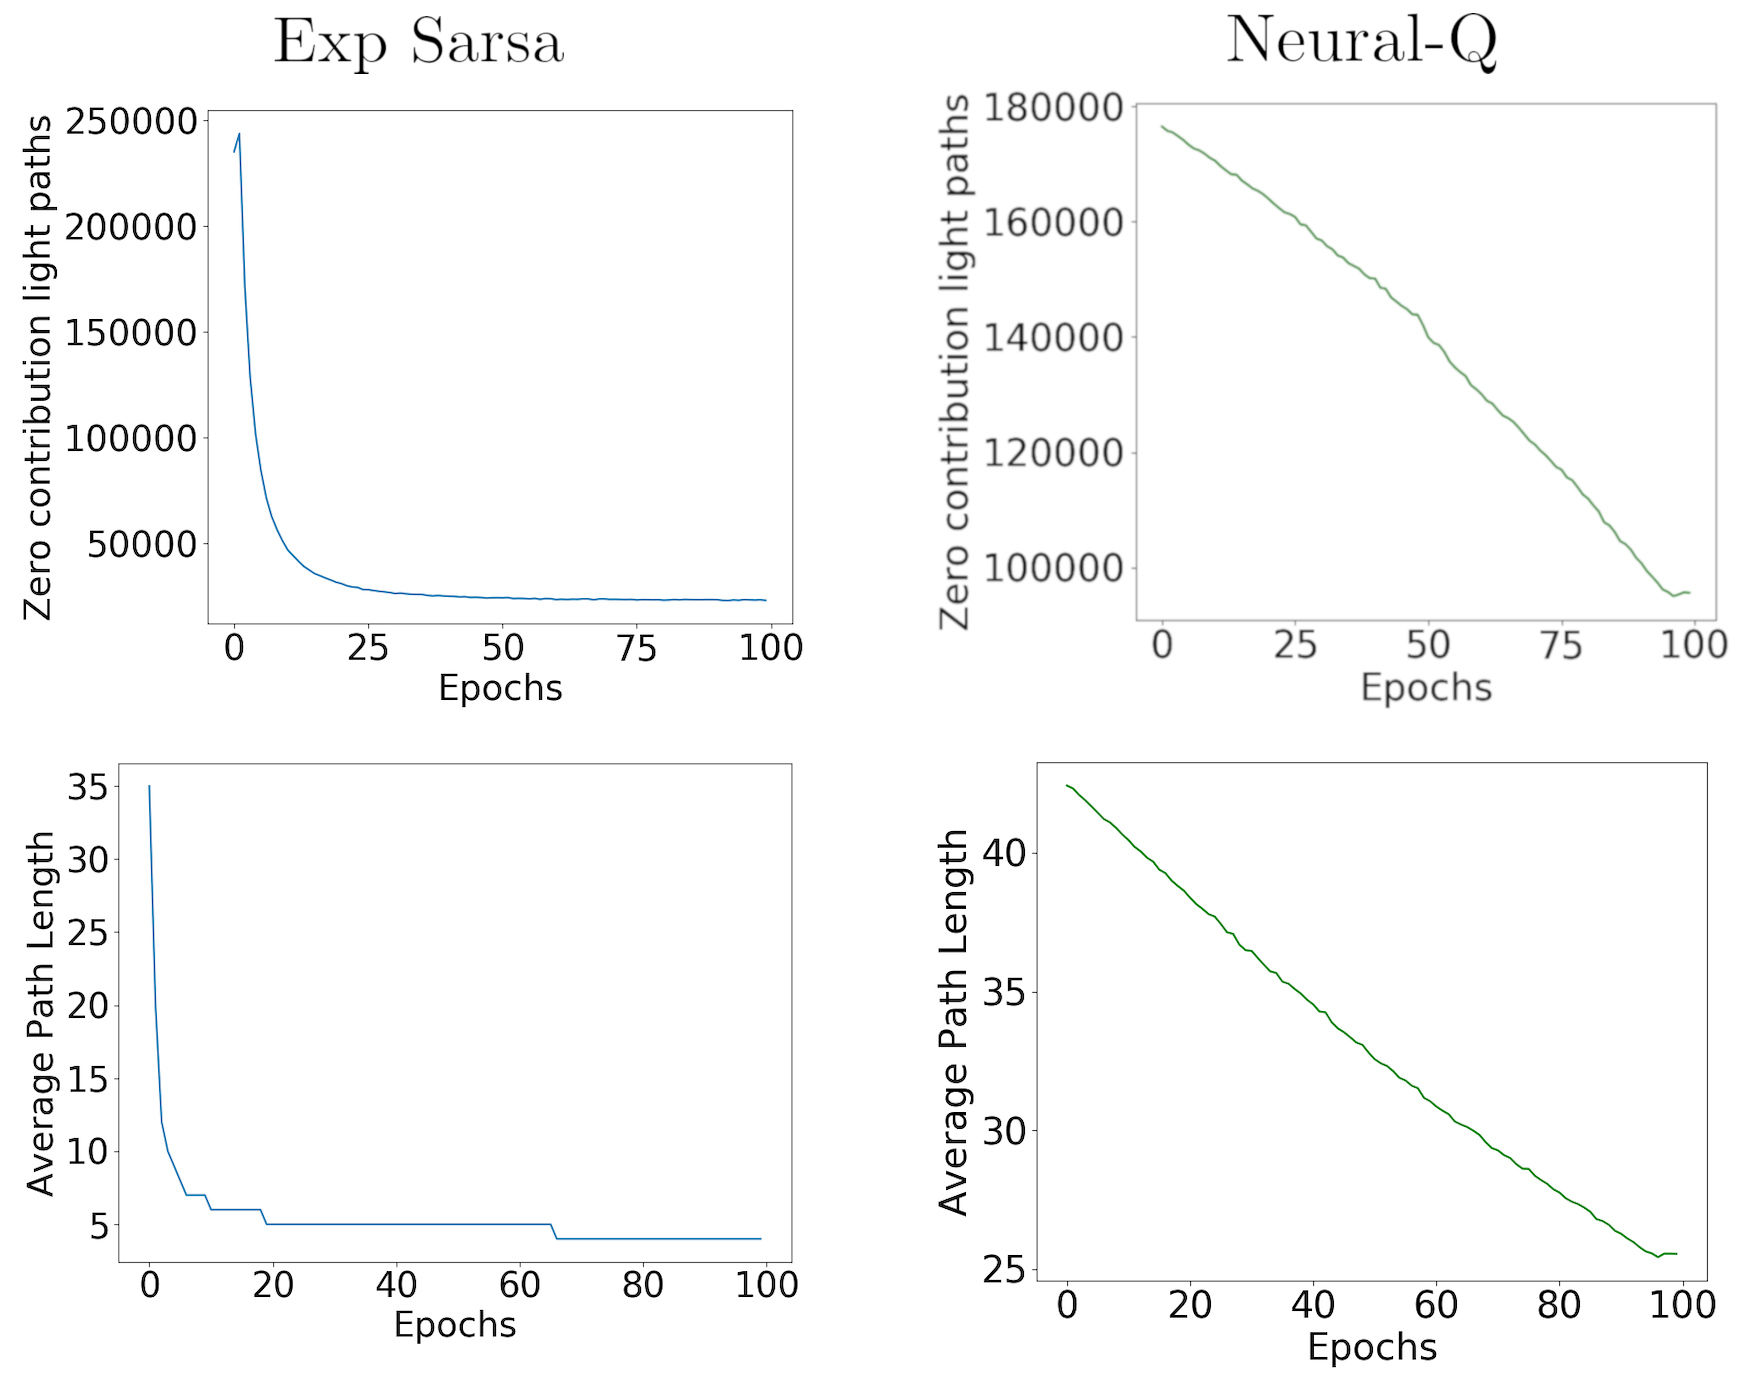
\includegraphics[width=0.6\textwidth]{images/training_curves.png}    
\end{center}
\caption{Training curves for the average path length and number of zero contribution light paths when rendering the Shelter scene for 100 epochs, using both the Expected Sarsa and Neural-Q path tracers. An epoch represents one sampled light ray through every pixel in the image. The average path length is the number reflections a light path takes before intersecting with a light source. A zero contribution light path is one which contributes almost zero colour to the final image.}
\label{fig:training_curves_archway}
\end{figure}


\begin{figure}[h]
\centering
\minipage{0.32\textwidth}
  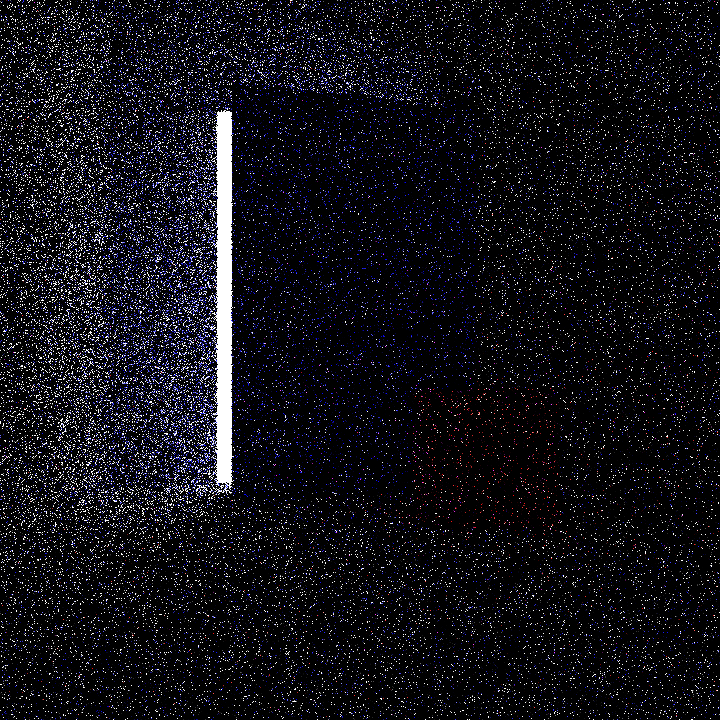
\includegraphics[width=\textwidth]{images/renders/max_dir/1_spp_default.png}   
  \subcaption{Default}\label{fig:default_1_spp}
\endminipage\hspace{0.1em}
\minipage{0.32\textwidth}
  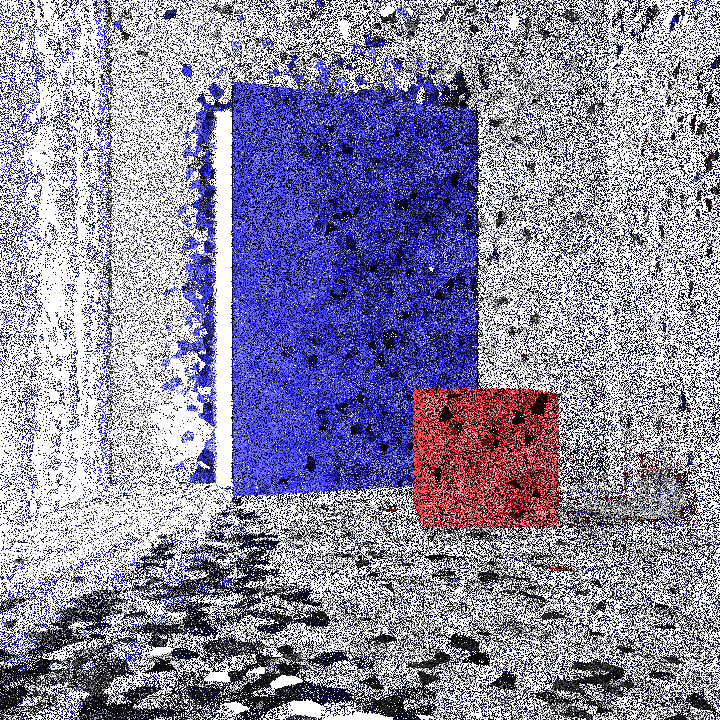
\includegraphics[width=\textwidth]{images/renders/max_dir/1_spp_sarsa_max_dir.png}   
  \subcaption{Expected Sarsa}\label{fig:sarsa_1_spp}
\endminipage\hspace{0.1em}
\minipage{0.32\textwidth}
  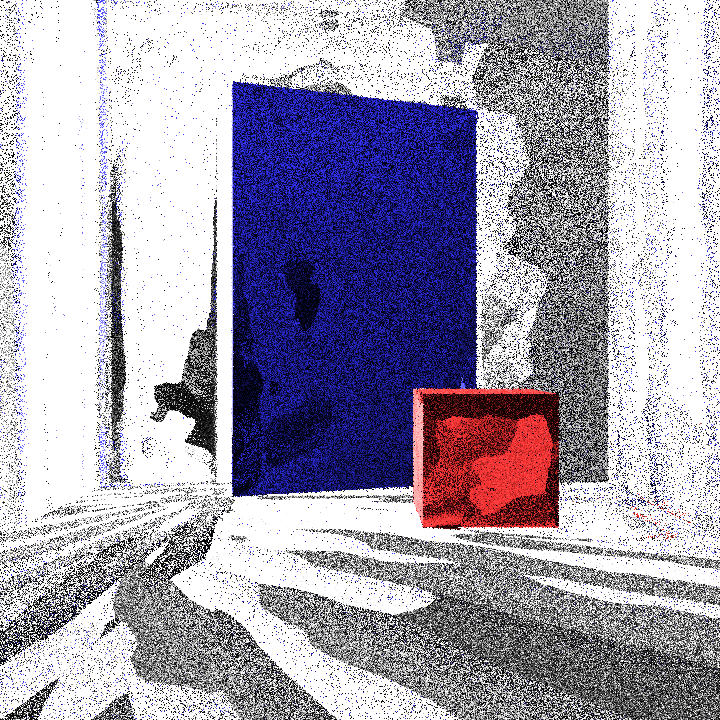
\includegraphics[width=\textwidth]{images/renders/max_dir/1_spp_nn_max_dir.png}
  \subcaption{Neural-Q}\label{fig:neural_q_1_spp}
\endminipage
\caption{The Door Room scene rendered using only 1 sampled light path per pixel with the default path tracer, a trained Expected Sarsa path tracer, and a trained Neural-Q path tracer. The light path through each pixel using the default path tracer is constructed according to Algorithm \ref{alg:default_path_tracer}. Whereas, the single sample for each pixel in the Expected Sarsa and Neural-Q renders is constructed by reflecting the light path in the direction of highest estimated radiance upon every intersection point, until the light is intersected.}
\label{fig:1_spp_max_dir}
\end{figure}

\subsection{Hyper Parameter Tuning}
\begin{itemize}
\item Hyperparams in expected sarsa include what the min of radiance distribution can be set to, the selection of the learning rate $\alpha$, the memory used for the scene...
\item Hyperparams for Neural-Q on the other hand are the epsilon start and epsilon decay
\end{itemize}

\subsection{Reusing Trained ANN for Different Scenes}
\begin{itemize}
\item Expected Sarsa cannot be reused for a slightly different scene whereas the Neural-Q path tracer can 
\item Show the Neural-Q path tracer ability to be reused
\end{itemize}


\section{From Memory Bound to Compute Bound}

Computational resources utilized by the path tracing algorithms introduced is a very important talking point when considering the potential to be integrated into renders used in industry such as \cite{georgiev2018arnold, christensen2018renderman, hyperion}. In particular any bounds imposed on the algorithm from current available hardware are the most important to consider, as rendering algorithms should be designed to give as much power to artists as possible to create and render any arbitrary scene of their choice. A detailed investigation on both highly optimised implementations of the Expected Sarsa and Neural-Q path tracers performance using current available hardware warrants a detailed investigation in itself. Instead for completeness, this section presents a high level analysis of how both memory usage and compute power limits their performance.

\subsection{Memory Usage}

The default forward path tracer is compute bound, meaning the only way to make the algorithm faster is by providing more compute power. For example by parallelizing the rendering process using a GPU with a quicker processor clock speed. On the other hand, the performance of the Expected Sarsa algorithm for reducing image noise has been found to be bound by the amount of RAM the algorithm has available to it from the  underlying hardware. This is due to the requirement of storing the Q-table in RAM which holds the approximated incident radiance values for a scene.\\

\subsubsection{Expected Sarsa}

The size of memory used by the Q-table is defined by the number of Irradiance Volumes sampled across the scenes geometry, as well as the number incident radiance values stored for the discrete directions $\omega_k$ $\forall k = 1,...,n$  within each Irradiance Volume. I have found the higher the number of sampled Irradiance Volumes the more accurate the incident radiance approximation is for a given intersection point, as shown in Figure \ref{fig:more_irradiance_volumes}.  I have found this is due to the average distance from a light path intersection point to the closest Irradiance Volume decreases as the number of Irradiance Volumes sampled in the scene increases. This becomes clear by observing Figure \ref{fig:voronoi_difference}, where the Voronoi plot of the scene with a lower number of sampled Irradiance Volumes on average has a larger sector size, meaning the nearest neighbour search on average will have a higher distance to each Irradiance Volume compared to that of the scene with more Irradiance Volumes. Recall that a nearest neighbour search is used to estimate the incident radiance on a point based on the stored values in the closest Irradiance Volume, therefore the closer the Irradiance Volume used for this approximation the more accurate the approximation of incident radiance on the point will be.\\

% Stats showing more samples for expected sarsa the better the approximation & images
% 1 image for more irradiance volumes -> showing the scene discretization
% 1 image for higher number of angles represented, the lower the MAPE score
%1 image showing artefacts from too low number of irradiance volumes
% Pics for increasing volumes and directions in volumes

A clear problem from this relationship is that if the underlying system does not have enough RAM, then the algorithm will not be able to significantly reduce the amount of noise in rendered images. Now, this may not be a problem for most small scenes with a polygon count ofaround 100, as common commodity graphics cards such as the NVIDIA 1070Ti GPU used for my experiments comes with 8GB of global memory (RAM), and NVIDIA claim they are able to fit the Q-table for a such scenes into only 2MB of memory to receive a significant reduction in noise \cite{dahm2017learning}. However, films commonly render scenes with hundred of thousands, or even millions of polygons potentially making it impossible to store a Q-table large enough to significantly reduce image noise in RAM. For example, in Transformers Revenge of the Fallen, the robot 'Devastator' was made out of 11,716,127 polygons \cite{devastator}. To present this memory scaling issue, Figure \ref{} presents a render of the Cornell Box scene which uses only xMB of memory to store the Q-table. The artefacts present in the image are cause by vastly incorrect importance\\

% Figure showing door room and complex light room with same amount of memory and showing how MAPE score is higher of other

\subsubsection{Neural-Q}

The Neural-Q path tracer on the other hand does not have exhibit the scaling in memory requirements as that of the Expected Sarsa path tracer. The is due to the Neural-Q path tracer only requiring more memory to store the incident radiance values for the current batch of light paths, which are used to importance sample directions for continuing the batch of light paths in. As well as, the amount of RAM required to store the ANN. The memory required to store the current batch of incident radiance values is controllable by the batch size parameter for the number of rays, therefore does not scale with the complexity of the scenes geometry. But a study from \cite{ren2013global} suggests more layers may be required in ANNs to approximate the incident radiance $L_i(x, \omega)$ for scenes with more complex geometry, meaning more memory is required to store more weight parameters of the network. However, further experimentation must be done to investigate the scaling of memory usage to scenes with thousands of vertices for the two rendering methods, by using a more optimised rendering engine then the one I have built. The renders presented in Figure \ref{fig:mape_results_grid} were produced using a constant ANN architecture as specified in \ref{sec:ann_architecture}, which required only 30MB of memory to store the ANN as well as intermediate values computed during a forward pass. Whilst the Expected Sarsa path tracer required the rendered scenes with different geometry to have significantly different Q-table sizes to reduce rendered image noise. This is due to the ANNs ability to generalize the approximated incident radiance over the 5D space formed by a position $x \in \mathbb{R}^3$ and direction $\omega \in \mathbb{R}^2$. Where a single weight in the ANN has the capacity to contribute to the approximated radiance of many positions and directions in the scene. Hence, an ANN with 2 hidden layers was able to make a good approximation of the incident radiance for any $(x, \omega)$ for all tested scenes. The Q-table on the other hand holds an individual value for each incident radiance estimate $(x,\omega)$, therefore the storage requirements rose for the scenes rendered with more complex geometry. For example, the Q-table required for the Expected Sarsa rendering of the large archway scene without any artefacts used 272MB of data storage, 9X more than that of the Neural-Q path tracer.


%TODO number of sectors in irradiance volumes and its effect
Moreover, the higher the number of discrete directions$n$ held in each Irradiance Volume, the more accurate the estimated radiance distribution at the given intersection point will be, see Figure \ref{fig:more_directions}. This is because the true radiance distribution at any point in the scene is continuous, so the more samples used in the Monte Carlo approximation of this probability density function (see section \ref{sec:td_light_transport}), the lower the approximation error due the law of large number in Equation \ref{eq:law_large_numbers}. 

\subsection{Parallel Processing}

For high quality, high frame rate rendering of scenes, rendering algorithms in general become very computationally demanding \cite{crockett1995parallel}. In order to facilitate this high level of performance, parallel computing must be used to distribute the computational workload. This pattern follows for both scanline renderers and ray-tracing renderers (which path tracing falls into) \cite{alerstam2008parallel, fatahalian2009data}. The default path tracing algorithm in particular is an embarrassingly parallel algorithm \cite{embarissingly_parallelizable}, as the task of finding the colour estimate of a single light path can be performed independently by a single process without any communication to other processes. A simple example of this is given in \cite{accelerated_ray_tracing}, whereby using GPU the process of rendering an image using an algorithm which closely resembles path tracing is split among many cores on a GPU. In industry path tracing algorithms take advantage of parallelism to an unprecedented scale, such as Disney's supercomputer for rendering full-length films using the Hyperion renderer \cite{hyperion}. Therefore, for any modified path tracing algorithm to gain industries attention it needs to be able to take fully advantage of parallel computing hardware.\\

\subsubsection{Expected Sarsa}

The Expected Sarsa path tracer is no longer as trivial to parallelize as the default forward path tracing algorithm due to the the first addition to the algorithm detailed in section \ref{sec:expected_sarsa_path_tracer}, where the incident radiance estimate for a given entry $Q(x,\omega_k)$ is updated after each intersection point is traced for constructing a light path. To parallelize the algorithm means to create and individual process to construct each light path as part of determining the estimate of a pixel value. However, the Q-table which stores the current approximation of all discrete incident radiance values in the scene is accessed by each thread. Meaning, it is possible that two threads will attempt to write to the same location at the same time in the Q-table if they intersect near one another, causing the update rule provided in Equation \ref{eq:mc_expected_sarsa_td_learning} will not be applied correctly. To remedy this, the update rule can be placed within a critical code section \cite{raynal2012concurrent} to ensure only one thread at a time can calculate and set the updated incident radiance estimate. For my purposes, all code written for parallel execution used the CUDA Toolkit \cite{cuda}, where CUDA atomic operations were used to ensure only one thread at a time can calculate and apply the Q-value update. The critical section added a minor performance overhead to each thread in both waiting to and performing the update rule. However it was negligible when using a Q-table near the size of any used to render the images in \ref{fig:mape_results_grid}, as due to the number of Q-values it is rare two threads attempt to write to the same address at the same time.\\ 

A significant performance penalty I found the Expected Sarsa method imposes on path tracing, is the time taken to perform the nearest neighbour search for finding the closest Irradiance Volume to a given intersection point in the scene. Whilst I implemented a KD-Tree on the GPU in order to reduce the nearest neighbour computational complexity to $O( \log n)$, I found the Expected Sarsa path tracer ran XX times slower then that of the default path tracer. The cause of this slowdown was found to be in per thread memory read times to global CUDA memory \cite{cuda_c_guide}. As a quick overview of CUDA's thread hierarchy; an execution thread in CUDA is contained within a group of threads known as a thread block. Each thread block is executed by a symmetric multiprocessor (SM) placed in a GRID. Following this, the memory hierarchy consists of per-thread local memory, per-block shared memory, and global memory which any thread can read and write to at any time. The issue with the Expected Sarsa path tracer is the Q-table is that the Q-table needs to be globally accessible to any thread in the GPU at any time, as every thread will be constructing a light path and during its construction it may update the value of any $Q(x, \omega)$ in the Q-table. This compounded with that the Q-table is far too large to store in per-thread or per-block memory for any commodity GPU, means nearest neighbour lookup performs $O(\log n)$ global memory lookups. Each uncached global memory lookup has roughly 100X higher latency then that of per-thread or per-block memory lookups \cite{global_vs_shared}. Hence, the Expected Sarsa algorithm experiences a high performance penalty from idle time waiting for data to be returned from global memory. Note, NVIDIA claims that the Expected Sarsa path tracer is able to render images with the same number of samples per pixel only 20\% then that of the default path tracer \cite{dahm2017learning} to significantly reduce image noise, however they do not specify the details of the machines that were running these experiments. My implementation could be further optimised by ensuring aligned memory access and reducing the amount of data retrieved, however it is unlikely that any of these optimisations will be able to avoid the bottleneck of regularly querying global memory.\\

\subsubsection{Neural-Q}

%TODO timing stats for training and tracing rays -> compared to expected sarsa as well
As for the Neural-Q path tracer parallel execution is slightly different, whereby batches of light paths colour estimates are computed once at a time. Note, the batch size should be set to be large enough such that no processors are idle whilst computing a batch, whilst being able to hold the temporary approximated incident radiance values in memory which are used for importance sampling directions to continue light paths in. Also, mini-batches which are the same size as the batch of light paths can be used in querying and training the ANN by stochastic gradient descent. A problem which added a significant performance penalty on my approach compared to that in \cite{muller2018neural}, is that there was no built in way to evaluate an ANN per-thread on the GPU using the Dynet framework, only code from the CPU could call any of the Dynet API functions. Meaning, my implementation had to frequently send data produced from tracing a batch of light paths to their next intersection point (positions, normals, throughputs etcetera) from the GPU to the CPU, only to call a dynet function which moved the data back to the GPU again for evaluating the ANN. Within Algorithm \cite{alg:neural_q_path_tracer} there are a total of $3$ calls to the Dynet API for evaluating the network for every batch of light ray paths, this means there is a total $6$ batch data transfers from the host device memory (that directly accessible by the CPU) to GPU memory, as illustrated in \ref{fig:memory_transfer}. \\

% Illustration of data transfers

The latency added by this design flaw is mainly due to the peak bandwidth available for transferring data between memory in the GPU is 144 GB/s, while for transferring data from the CPU to the GPU (and vice versa) is only 8 GB/s \cite{global_data_transfer}. Therefore, the 18x performance penalty received $6$ times with each batch computation, makes evaluating my implementation of the Neural-Q path tracer on render time not a fair test. However, the performance penalty received by methods which use neural network based importance sampling for Monte Carlo path tracing have found that the cost of the evaluating the ANN without the data transfers from CPU to GPU (and vice verca) can still add a 10X peformance penalty compared to other importance sampling methods in some cases \cite{muller2018neural, keller2019integral}. Clearly this needs to be alleviated before the neural network importance sampling methods are adopted for Monte Carlo path tracing in industry. Answers to this problem may already lie in existing hardware, by leveraging the power of NVIDIAS TensorCores in Tesla GPUs \cite{tensor_cores}, which claims to have 40X higher performance than CPUs for inference on ANNs.


\section{Neural-Q Path Tracer Design}
Move section down here discussing other methods

\begin{itemize}
\item With and without vertices in coord space for training and state reasoning
\item Number of actions experimented with on door scene
\item With and without epsilon greedy, lack of exploration
\end{itemize}

\section{Recent Advancements in Neural Importance Sampling for Monte Carlo Path Tracing}

Along with Nvidia's paper which suggested a reinforcement learning approach for approximating the incident radiance at any point in a scene \cite{dahm2017learning}, other reinforcement learning based methods for learning light transport in a scene have been engineered \cite{muller2017practical, vorba2014line}, but none of them investigated the potential of deep reinforcement learning for this problem. However, recently neural networks for both the global and local sampling for light path construction have had a large amount of research \cite{zheng2018learning, muller2018neural, keller2019integral, hermosilla2018deep}. Global light path sampling is where the optimal density of sampled light rays per pixel is determined by the learning algorithm. Therefore, the reinforcement learning agent only determines where light paths should initially be sampled from. While this method does not reduce noise in the Monte Carlo path tracing to the extent local importance sampling does, both \cite{muller2017practical, zheng2018learning} have applied this technique to reduce image noise with a much lower performance penalty compared to that of local importance sampling. I however, work on evaluating local light path sampling methods. Local light path sampling involves learning directions to continue light paths in when they intersect with surfaces in the scene, to efficiently guide them towards light sources.\\

 The follow up paper to the one which introduced the Expected Sarsa path tracer \cite{dahm2017learning} is \cite{keller2019integral}. Here, ANNs are experimented with for rendering in three different ways; for a given intersection point in the scene an ANN is trained to determine which light source should be used to compute the direct light incident on that intersection point, for approximating the visibility of an intersection point to all light sources, and for approximating the radiance at a given point in the scene to directly approximate a pixels colour value using many small ANNs. The results are promising for all three use cases, however unlike the Neural-Q path tracer, none of the methods estimate the incident radaince from a set of discrete directions around a point for importance sampling.\\
 
 Another paper published by Disney's Zurich research team during the implementation of this thesis in Febuary 2019 introduced neural importance sampling \cite{muller2018neural}, which samples a direction to continue a light path in and is known as Neural Path Guiding (NPG). This is currently the only other method which is an alternative for using neural networks to importance sample directions to continue light paths in. An ANN framework for modelling complex high-dimensional densities known as Non-linear independent Component Estimation (NICE) \cite{dinh2014nice} is trained to learn the distribution of incident radiance at any given point in the scene. However, unlike my approach, the network takes in the intersection point $x \in \mathbb{R}^3$, intersection surface normal and the outgoing direction $\omega_o$ of interest to directly evaluate $L_o(x, \omega_o)$. A one blob encoding is then applied to these inputs which improves the speed and performance of inference by the network to output a single direction $\omega$ to continue the light path in. The probability density function over the hemisphere $\Omega$ of possible directions to sample from at an intersection point $x$ can also be evaluated at $\omega$ using the proposed ANN framework. This has the advantage over my approach as it is able to learn the radiance distribution over the continuous set of directions in a hemisphere around the intersection point. Rather than discretizing the hemisphere into an adaptive quadrature to represent the radiance distribution as a discrete set of directions $omega_k$ $\forall i = 0, ..., n$. However, the ANN framework proposed is far more expensive to evaluate than that used by the Neural-Q path tracer as it consisting of a one-blob encoding, many fully connected layers and a piecewise polynomial warp \cite{muller2018neural}. Whereas, the Neural-Q network in comparison only consists of two hidden layers, hence requires less memory for storing parameter values and evaluating the network compared to that in \cite{muller2018neural}. A comparison between the NPG and Neural-Q path tracers for their ability to reduce noise in Monte Carlo path tracing is an interesting area for future investigation.

\begin{comment}

{\bf A topic-specific chapter, of roughly $15$ pages} 
\vspace{1cm} 

\noindent
This chapter is intended to evaluate what you did.  The content is highly 
topic-specific, but for many projects will have flavours of the following:

\begin{enumerate}
\item functional  testing, including analysis and explanation of failure 
      cases,
\item behavioural testing, often including analysis of any results that 
      draw some form of conclusion wrt. the aims and objectives,
      and
\item evaluation of options and decisions within the project, and/or a
      comparison with alternatives.
\end{enumerate}

\noindent
This chapter often acts to differentiate project quality: even if the work
completed is of a high technical quality, critical yet objective evaluation 
and comparison of the outcomes is crucial.  In essence, the reader wants to
learn something, so the worst examples amount to simple statements of fact 
(e.g., ``graph X shows the result is Y''); the best examples are analytical 
and exploratory (e.g., ``graph X shows the result is Y, which means Z; this 
contradicts [1], which may be because I use a different assumption'').  As 
such, both positive {\em and} negative outcomes are valid {\em if} presented 
in a suitable manner.

\subsection{Plan}

\textbf{Data to collect}
\begin{itemize}

\item Build 4 different scenes:

\begin{itemize}
\item Simple geometry, Indirectly illuminated scene: Here both reinforcement learning methods should perform excellently

\item Simple geometry, Directly illuminated scene: Here all methods should perform well

\item Complex geometry, Indirectly illuminated scene: Can both methods do this - will take a lot of training, deeper NN potentially

\item Complex geometry, Directly illuminated scene: Can both methods do this - will take a lot of training, deeper NN potentially
\end{itemize}

\item Number zero-contribution light paths/ light paths that do not intersect with a with a light after $n$ bounces therefore they become irrelevant for all methods with accumulated frames on the x-axis

\item Variance in points around the room to train network in order to make training batches as varied as possible (this is a weird one, essentially assessing the fact that we do not need a replay buffer).

\item eta-greedy constant for loss curve for training the network \& decaying eta-greedy policy graph for the loss as well

\item Visual representation of Q-values being higher in directions near light source: Map q-values to hemispheres in the scene and get a close up, clearly indicating its ability to sample in the correct direction

\item 1 SPP, 16 SPP, 32 SPP, 64 SPP, 128 SPP, 256 SPP for all three methods on 4 different scenes to evaluate their effectiveness: Assessing accuracy of global illumination approximation

\item Limitations: Number of angles which can accurately be learned by the network, accuracy  needs to be compared with expected SARSA approach for a single radiance volume at a given point in the scene. Size of the scene which can be learnt accurately.

\end{itemize}

\textbf{Preliminary}
\begin{enumerate}
\item Exploration vs Exploitation for both techniques, exploration can yield to better results plus exploitation does not accurately simulate light, relate to the rendering equation and how light works in the physical world.

\item Show for about 4 different scenes the results for a $n$ different numbers of samples; the images, average path length, number of light paths which actually contribute to the image which are sampled between all techniques. I will have to analyse which reduces the number of zero contribution paths the most, but also still assess if the image is photo-realistic.

\item Also analyse default Q-learnings ability on top of expected SARSA

\item Justify reasoning for choosing to analyse Q-Learning, Expected SARSA and DQN (because they have good results for other cases and TD learning fits the online learning procedure)

\item Assess the number of parameters required, configuration is important for these algorithms, if it is very difficult to get right, then the time spent configuring may not be worth it compared to actually rendering the image. E.g. default path-tracing there are not other parameters apart from the number of samples per pixel, expected SARSA requires the user to specify the memory which is allowed to be used by the program, this requires careful consideration, as well as the threshold the distribution cannot fall below, the deep Q-learning algorithm requires less config but potentially different neural network architectures should be investigated to further reduce the number of zero-contribution light paths. 

\item Ease of implementation 

\item Parallelisability of each algorithm, path-tracing is far easier to parallelise as it requires minimal memory accesses by the program to infer pixel values, as opposed to expected SARSA which requires many. Deep-q learning has more customizability in terms of parallelizing (needs more research)

\item Memory usage: Path-tracing is minimal, Expected SARSA is unbounded, Deep Q-Learning is bounded by the size of the neural network, but the memory it requires is still significant (needs more research)

\item DQN vs Expected Sarsa: Do not have to wait for an iteration to begin
 importance sampling on the newly learned Q values for a given point, 
 neural network is continually trained and inferred from. Continuous state 
 space vs discretized required for storage in expected SARSA.
\end{enumerate}

\end{comment}

\end{document}